% -*- Mode:TeX -*-

%% IMPORTANT: The official thesis specifications are available at:
%%            http://libraries.mit.edu/archives/thesis-specs/
%%
%%            Please verify your thesis' formatting and copyright
%%            assignment before submission.  If you notice any
%%            discrepancies between these templates and the 
%%            MIT Libraries' specs, please let us know
%%            by e-mailing thesis@mit.edu

%% The documentclass options along with the pagestyle can be used to generate
%% a technical report, a draft copy, or a regular thesis.  You may need to
%% re-specify the pagestyle after you \include  cover.tex.  For more
%% information, see the first few lines of mitthesis.cls. 

%\documentclass[12pt,vi,twoside]{mitthesis}
%%
%%  If you want your thesis copyright to you instead of MIT, use the
%%  ``vi'' option, as above.
%%
%\documentclass[12pt,twoside,leftblank]{mitthesis}
%%
%% If you want blank pages before new chapters to be labelled ``This
%% Page Intentionally Left Blank'', use the ``leftblank'' option, as
%% above. 

\documentclass[12pt,twoside]{mitthesis}
\usepackage{lgrind}
\usepackage{graphicx}
%% These have been added at the request of the MIT Libraries, because
%% some PDF conversions mess up the ligatures.  -LB, 1/22/2014
\usepackage{cmap}
\usepackage[T1]{fontenc}
\usepackage{subcaption}
\usepackage{tikz,pgfplots}

\pagestyle{plain}

%% This bit allows you to either specify only the files which you wish to
%% process, or `all' to process all files which you \include.
%% Krishna Sethuraman (1990).

%%\typein [\files]{\include{all}}
%%\def\all{all}
%%\ifx\files\all \typeout{Including all files.} \else \typeout{Including only \files.} \includeonly{\files} \fi

\newlength\figureheight 
\newlength\figurewidth 

\begin{document}

% -*-latex-*-
% 
% For questions, comments, concerns or complaints:
% thesis@mit.edu
% 
%
% $Log: cover.tex,v $
% Revision 1.8  2008/05/13 15:02:15  jdreed
% Degree month is June, not May.  Added note about prevdegrees.
% Arthur Smith's title updated
%
% Revision 1.7  2001/02/08 18:53:16  boojum
% changed some \newpages to \cleardoublepages
%
% Revision 1.6  1999/10/21 14:49:31  boojum
% changed comment referring to documentstyle
%
% Revision 1.5  1999/10/21 14:39:04  boojum
% *** empty log message ***
%
% Revision 1.4  1997/04/18  17:54:10  othomas
% added page numbers on abstract and cover, and made 1 abstract
% page the default rather than 2.  (anne hunter tells me this
% is the new institute standard.)
%
% Revision 1.4  1997/04/18  17:54:10  othomas
% added page numbers on abstract and cover, and made 1 abstract
% page the default rather than 2.  (anne hunter tells me this
% is the new institute standard.)
%
% Revision 1.3  93/05/17  17:06:29  starflt
% Added acknowledgements section (suggested by tompalka)
% 
% Revision 1.2  92/04/22  13:13:13  epeisach
% Fixes for 1991 course 6 requirements
% Phrase "and to grant others the right to do so" has been added to 
% permission clause
% Second copy of abstract is not counted as separate pages so numbering works
% out
% 
% Revision 1.1  92/04/22  13:08:20  epeisach

% NOTE:
% These templates make an effort to conform to the MIT Thesis specifications,
% however the specifications can change.  We recommend that you verify the
% layout of your title page with your thesis advisor and/or the MIT 
% Libraries before printing your final copy.
\title{Autonomous Grasping of Dynamic Objects}

\author{Patrick Lynch}
% If you wish to list your previous degrees on the cover page, use the 
% previous degrees command:
%       \prevdegrees{A.A., Harvard University (1985)}
% You can use the \\ command to list multiple previous degrees
%       \prevdegrees{B.S., University of California (1978) \\
%                    S.M., Massachusetts Institute of Technology (1981)}
\department{Department of Mechanical and Manufacturing Engineering}

% If the thesis is for two degrees simultaneously, list them both
% separated by \and like this:
% \degree{Doctor of Philosophy \and Master of Science}
\degree{Bachelor of Science in Computer Science and Engineering}

% As of the 2007-08 academic year, valid degree months are September, 
% February, or June.  The default is June.
\degreemonth{June}
\degreeyear{1990}
\thesisdate{May 18, 1990}

%% By default, the thesis will be copyrighted to MIT.  If you need to copyright
%% the thesis to yourself, just specify the `vi' documentclass option.  If for
%% some reason you want to exactly specify the copyright notice text, you can
%% use the \copyrightnoticetext command.  
%\copyrightnoticetext{\copyright IBM, 1990.  Do not open till Xmas.}

% If there is more than one supervisor, use the \supervisor command
% once for each.
\supervisor{Dr Conor McGinn}{Assistant Professor}

% This is the department committee chairman, not the thesis committee
% chairman.  You should replace this with your Department's Committee
% Chairman.
\chairman{Arthur C. Smith}{Chairman, Department Committee on Graduate Theses}

% Make the titlepage based on the above information.  If you need
% something special and can't use the standard form, you can specify
% the exact text of the titlepage yourself.  Put it in a titlepage
% environment and leave blank lines where you want vertical space.
% The spaces will be adjusted to fill the entire page.  The dotted
% lines for the signatures are made with the \signature command.
\maketitle

% The abstractpage environment sets up everything on the page except
% the text itself.  The title and other header material are put at the
% top of the page, and the supervisors are listed at the bottom.  A
% new page is begun both before and after.  Of course, an abstract may
% be more than one page itself.  If you need more control over the
% format of the page, you can use the abstract environment, which puts
% the word "Abstract" at the beginning and single spaces its text.

%% You can either \input (*not* \include) your abstract file, or you can put
%% the text of the abstract directly between the \begin{abstractpage} and
%% \end{abstractpage} commands.

% First copy: start a new page, and save the page number.
\cleardoublepage
% Uncomment the next line if you do NOT want a page number on your
% abstract and acknowledgments pages.
% \pagestyle{empty}
\setcounter{savepage}{\thepage}
\begin{abstractpage}
% $Log: abstract.tex,v $
% Revision 1.1  93/05/14  14:56:25  starflt
% Initial revision
% 
% Revision 1.1  90/05/04  10:41:01  lwvanels
% Initial revision
% 
%
%% The text of your abstract and nothing else (other than comments) goes here.
%% It will be single-spaced and the rest of the text that is supposed to go on
%% the abstract page will be generated by the abstractpage environment.  This
%% file should be \input (not \include 'd) from cover.tex.

% should be ~500 words

%% Background
Grasping moving objects is a challenging problem in the field of robotics. Traditional approaches are computationally expensive, over reliant on vision-based systems and often require an existing sensor infrastructure in the robot's environment. These make existing techniques unsuitable for implementation on mobile robotic platforms. The potential contribution of alternative strategies, in particular of other types of sensing, remains under-explored. 
%% Aims
The aim of this project is to investigate the role which sensing plays in the ability of a robot to grasp an object in motion. It is hypothesised that a sensor-heavy approach, where multiple sensing modalities are combined, can enable a robust grasping strategy, suited to implementation on a mobile robot.
%% Method
In order to test this hypothesis, the topic was broken into several research questions and addressed individually. In order to enable testing, a two-finger pincer gripper was designed and manufactured. To date, tests were performed on this pincer gripper with and without tactile sensing and their performances compared. A similar methodology will be employed in the future to investigate other sensing mechanisms, including vision and remote tactile.
%% Results and Conclusion
Tests have found that tactile feedback provided in real-time enabled the gripper to rapidly adapt to the moving object. This resulted in higher observed grasp robustness, in particular when the object's trajectory was offset from the center of the gripper. These findings indicate that tactile sensing can play an important role in informing the gripper motion when grasping moving objects and motivates further research on how the contribution of tactile sensing can be optimised and what other types of sensing might be utilised in creating a sensor-informed grasping motion for autonomous grasping of moving objects.

% conclusion, comment, contribution
% how have you added to field?




\end{abstractpage}

% Additional copy: start a new page, and reset the page number.  This way,
% the second copy of the abstract is not counted as separate pages.
% Uncomment the next 6 lines if you need two copies of the abstract
% page.
% \setcounter{page}{\thesavepage}
% \begin{abstractpage}
% % $Log: abstract.tex,v $
% Revision 1.1  93/05/14  14:56:25  starflt
% Initial revision
% 
% Revision 1.1  90/05/04  10:41:01  lwvanels
% Initial revision
% 
%
%% The text of your abstract and nothing else (other than comments) goes here.
%% It will be single-spaced and the rest of the text that is supposed to go on
%% the abstract page will be generated by the abstractpage environment.  This
%% file should be \input (not \include 'd) from cover.tex.

% should be ~500 words

%% Background
Grasping moving objects is a challenging problem in the field of robotics. Traditional approaches are computationally expensive, over reliant on vision-based systems and often require an existing sensor infrastructure in the robot's environment. These make existing techniques unsuitable for implementation on mobile robotic platforms. The potential contribution of alternative strategies, in particular of other types of sensing, remains under-explored. 
%% Aims
The aim of this project is to investigate the role which sensing plays in the ability of a robot to grasp an object in motion. It is hypothesised that a sensor-heavy approach, where multiple sensing modalities are combined, can enable a robust grasping strategy, suited to implementation on a mobile robot.
%% Method
In order to test this hypothesis, the topic was broken into several research questions and addressed individually. In order to enable testing, a two-finger pincer gripper was designed and manufactured. To date, tests were performed on this pincer gripper with and without tactile sensing and their performances compared. A similar methodology will be employed in the future to investigate other sensing mechanisms, including vision and remote tactile.
%% Results and Conclusion
Tests have found that tactile feedback provided in real-time enabled the gripper to rapidly adapt to the moving object. This resulted in higher observed grasp robustness, in particular when the object's trajectory was offset from the center of the gripper. These findings indicate that tactile sensing can play an important role in informing the gripper motion when grasping moving objects and motivates further research on how the contribution of tactile sensing can be optimised and what other types of sensing might be utilised in creating a sensor-informed grasping motion for autonomous grasping of moving objects.

% conclusion, comment, contribution
% how have you added to field?




% \end{abstractpage}

\cleardoublepage

\section*{Acknowledgments}

This is the acknowledgements section.  You should replace this with your
own acknowledgements.

%%%%%%%%%%%%%%%%%%%%%%%%%%%%%%%%%%%%%%%%%%%%%%%%%%%%%%%%%%%%%%%%%%%%%%
% -*-latex-*-

% Some departments (e.g. 5) require an additional signature page.  See
% signature.tex for more information and uncomment the following line if
% applicable.
% % -*- Mode:TeX -*-
%
% Some departments (e.g. Chemistry) require an additional cover page
% with signatures of the thesis committee.  Please check with your
% thesis advisor or other appropriate person to determine if such a 
% page is required for your thesis.  
%
% If you choose not to use the "titlepage" environment, a \newpage
% commands, and several \vspace{\fill} commands may be necessary to
% achieve the required spacing.  The \signature command is defined in
% the "mitthesis" class
%
% The following sample appears courtesy of Ben Kaduk <kaduk@mit.edu> and
% was used in his June 2012 doctoral thesis in Chemistry. 

\begin{titlepage}
\begin{large}
This doctoral thesis has been examined by a Committee of the Department
of Chemistry as follows:

\signature{Professor Jianshu Cao}{Chairman, Thesis Committee \\
   Professor of Chemistry}

\signature{Professor Troy Van Voorhis}{Thesis Supervisor \\
   Associate Professor of Chemistry}

\signature{Professor Robert W. Field}{Member, Thesis Committee \\
   Haslam and Dewey Professor of Chemistry}
\end{large}
\end{titlepage}


\pagestyle{plain}
% -*- Mode:TeX -*-
%% This file simply contains the commands that actually generate the table of
%% contents and lists of figures and tables.  You can omit any or all of
%% these files by simply taking out the appropriate command.  For more
%% information on these files, see appendix C.3.3 of the LaTeX manual. 
\tableofcontents
\newpage
\listoffigures
\newpage
\listoftables


%% This is an example first chapter.  You should put chapter/appendix that you
%% write into a separate file, and add a line \include{yourfilename} to
%% main.tex, where `yourfilename.tex' is the name of the chapter/appendix file.
%% You can process specific files by typing their names in at the 
%% \files=
%% prompt when you run the file main.tex through LaTeX.

% make sure to keep this 2-5 pages

\chapter{Introduction}
Advances in robotic technology have enabled a continuous increase in what a robot is capable of. A constantly growing range of features is increasing the potential usefulness of robotic technology. Robots have already been widely adapted in industrial applications for automation and are becoming increasingly ubiquitous in a wider range of applications. Service robots are one example of this, it is increasingly common to see robots in entertainment, hospitality and health care applications.There are huge advantages to expanding robotic applications into these areas. To name just two examples, robots can be used to massively increase the independence of older adults or people living with disabilities and robots can carry out repetitive, and tedious jobs without boredom affecting their performance. With this ever expanding range of potential application however, new challenges are presented. 

% This paragraph needs rewritten and much of it rephrased and eloborated on

Robots, even relatively primitive robotic platforms, perform very well in the automation of manufacturing and assembly of products in industry and have done for several decades now. This is mainly due to the environment, which, in the case of manufacturing or assembly, is highly controlled and designed specifically for the robot in question. A robot used in automated assembly does not need to be adaptable, it will never have to work in different lighting conditions, or need to move to pick up something which is outside of it's manipulator's range, and it does not have to consider that something, for example a human, might get in the path of its arm. This is not true of robots which are designed to work in less structured environments. A robot working in a hotel, building lobby or health care facility needs to be much more adaptable, this adaptability requires a much higher level of complexity. There is a demand, even within industrial applications, for a more flexible and adaptable robot.  

One area where this move to more unstructured and dynamic environments is particularly challenging is manipulation and grasping. Grasping is an essential function of a general purpose robot. The ability to grasp and manipulate an object extends the robot's ability beyond sensing and navigating its environment to being able to manipulate and interact with it's environment, this massively increases its potential. In a more controlled environment when a robot grasps an object, very often the problem is vastly simplified by ensuring the object is in a known location and in a favourable orientation. When a robots needs to be able to effectively grasp in less structured environment this is not the case. For example, when the robot is more general purpose the range of objects which it will need to have the ability to grasp is much larger. More than just the size of the object will change, but also the shape and weight too. Furthermore, it is naive to assume that the objects which you will want to grasp will always be static and remain static throughout the interaction. This is where the focus of this research lays, this document outlines ongoing research which specifically examines the autonomous robotic grasping of dynamic objects.

\section{Background}

Robotic manipulation refers to a robots ability to manipulate its object in its environment. It is the robotic equivalent a humans hands and arms. This research focuses specifically on the end effector or gripper of the robot. This refers to the mechanism at the end of a robotic arm.

A vital part of grasping any object is the ability to localise it in space. The robot much have information about the relative pose, positions and velocities, of the object and itself. This can be achieved through the use of sensors, both sensing the external world, i.e. visual cameras and depth cameras and those monitoring the state of the robot, i.e. joint sensing, etc. The data collected, when processed can yield the necessary relative pose of robot and object as well as other information about the environment which may be relevant, i.e. possible collisions, etc. The success of this approach is dependant on everything from the lighting conditions and the shape of the object to the algorithm used.

This is further complicated in this work since we are trying to grasp a moving object. This uses a similar approach to locating a static object however it will do it across consecutive frames and collect data about the movement of the object, for example the velocity vector. One example predictive model is a simple linear projection of the balls position at time tnow+time to intercept, based on its current speed and direction.

new position = old position + speed * time to intercept

This research will also explore how further information about the movement of the object might help to inform the predictive model, i.e. a ball rolling down an inclined plane will require a different predictive model than a ball flying through three dimensional space.  

\subsection{Gripper}
The gripper is an essential part of this system, a well designed gripper could massively decrease the demands on other parts of the system, for example the accuracy of the intercept from the predictive model. A poorly designed gripper on the other hand may be fundamentally incapable of grasping a moving object regardless of the rest of the system. For this reason, a robotic grasper was developed specifically for grasping a dynamic object. This design was then validated experimentally and important design features where isolated and their value assessed. This experiment and the corresponding results are outlined below.

\subsection{Sensing}
Effective sensing is vital for any robotic system, sensors are how robots collect information about the world around it, they allow them to model, manipulate and react to their environment. In this research there is particular focus on two types of sensing, tactile and visual.

Visual sensing in this application is used for the localisation of the object and for the predictive model. Vision processing algorithms are implemented used OpenCV.

Tactile sensing is embedded in the hand and is used to inform the control of the hand enabling a smarter grasping strategy.


% research questions
\section{Research Questions}
\begin{itemize}
\item Can a vision based predictive model operate at a sufficiently high frame rate to allow an effective object interception % This can be answered by looking at prior art

\item Is there an approach to the predictive model which always performs best or do we need further information about the potential behaviour of the object % This is essentially trivial, It its fair to assume that more information about the behaviour will lead to a better predictive model

\item Can a manipulator, gripper system react sufficiently fast to information provided by a predictive model to grasp a moving object % Change this to refer to sensing, what modes of sensing give inform which is useful to inform the grasp

\item What features of a gripper design facilitate the grasping of a moving object %More specific about features

\item Can embedded tactile sensing enable a smarter grasping strategy and offer an increase in successful grasp % Too similar to the point above
\end{itemize}

% aims and hypothesis
\section{Aims and Objectives}
The primary aims of this research include:

\begin{itemize}
\item Present gazebo simulations which comparing the effectiveness of different approaches to predictive modelling of a dynamic object in different situations.
\item Present the results of experimental testing, conducted to examine how different features of a gripper contribute to a grippers ability to grasp a moving object.
\item Present a grasping strategy for the control of robot fingers based on feedback from embedded tactile sensors
\item Present gazebo simulations of effective visual servoing 
\end{itemize}

% aims 

% research contributions

% objectives



% document outline
\section{Document Outline}
Chapter 2 will present a comprehensive outline of the existing research and associated literature relevant to this challenge and give a sense of the current state of the art. Chapter 3 will explore predictive modelling of the dynamic object. This will be done in simulation where, several different approaches can be applied to a range of situations relatively quickly. Chapter 4 will present controlled experiments and corresponding results of robot grippers ability to grasp objects, different features of the gripper design are isolated and their contribution to the grasp assessed. Chapter 5 will look at sensing, both tactile and visual. The range of possibilities of each are explored and their value assessed. Finally Chapter 6 will conclude this transfer report, summing up the finding to date and outlining future work for this research project.




\chapter{Literature Review}



\section{Current State of the Art in grasping} % Not a good title!
Looking at recent demos for grasping functionality , including industrial applications. Everything presented should be at application and implementation stage.

\section{Existing platforms}

\subsection{Grippers}
There are a huge number of robotic gripper available both commercially and open source versions. These gripper vary widely from simplistic to very complex and from general purpose to having a very specific niche applications for which they were designed. It would be very difficult to complete a comprehensive review of all available grippers but this section introduces a subset, representative of the range of grippers developed to date. Grippers are generalised into categories based on their morphologies and real world examples of each are given.

\begin{itemize}
    \item Pincer Grippers \ref{fig:YouBot}, \ref{label:Robotiq85}, \ref{label:Hand-E}
    
    Pincer Grippers are one of the simplest types of gripper, but despite their simplicity they are capable of a wide range of tasks. This low complexity and large range of applications is why they are one of the most used gripper designs. Pincer gripper use 2 opposing fingers to apply a clamping force onto the object. They require low control complexity but can encounter problems if the object is too heavy or irregularly shaped.
    
    \item Higher DOF Finger grippers \ref{lbel:Robotiq3Finger}
    \item Humanoid Grippers \ref{fig:Sandia}, \ref{fig:James}, \ref{fig:Allegro}, \ref{fig:DLR Hand II}
    \item Suction Cup Grippers
    \item Other \ref{fig:Coffee Bean Gripper}
\end{itemize}

\begin{figure}
    \centering
    \begin{subfigure}{.3\linewidth}
        \centering
        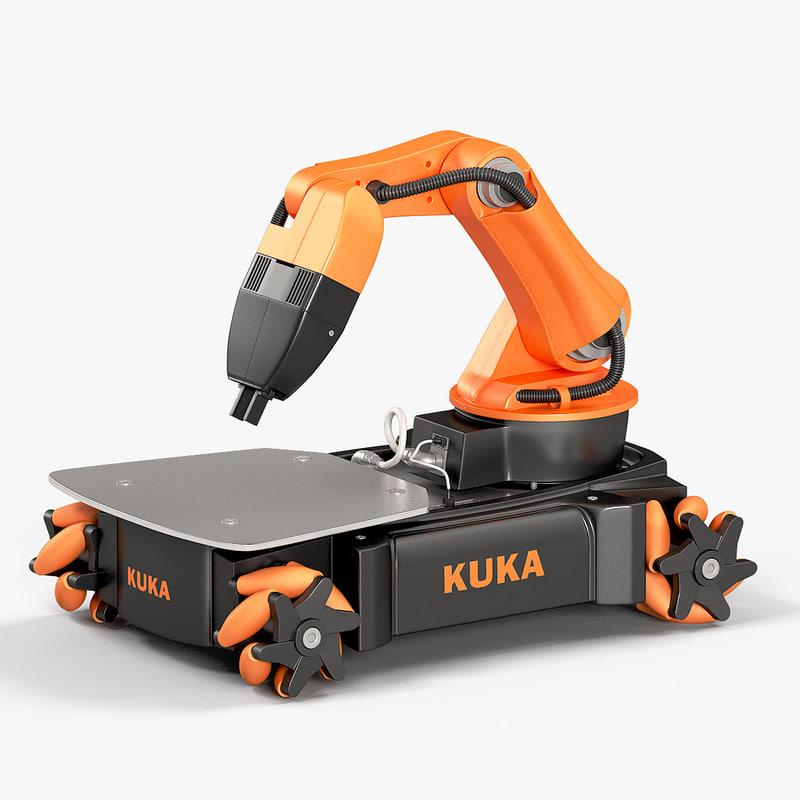
\includegraphics[width=0.7\textwidth]{Images/kuka-youbot-3D-model_0.jpg}
        \caption{YouBot}
        \label{fig:YouBot}
    \end{subfigure}
    \begin{subfigure}{.3\linewidth}
        \centering
        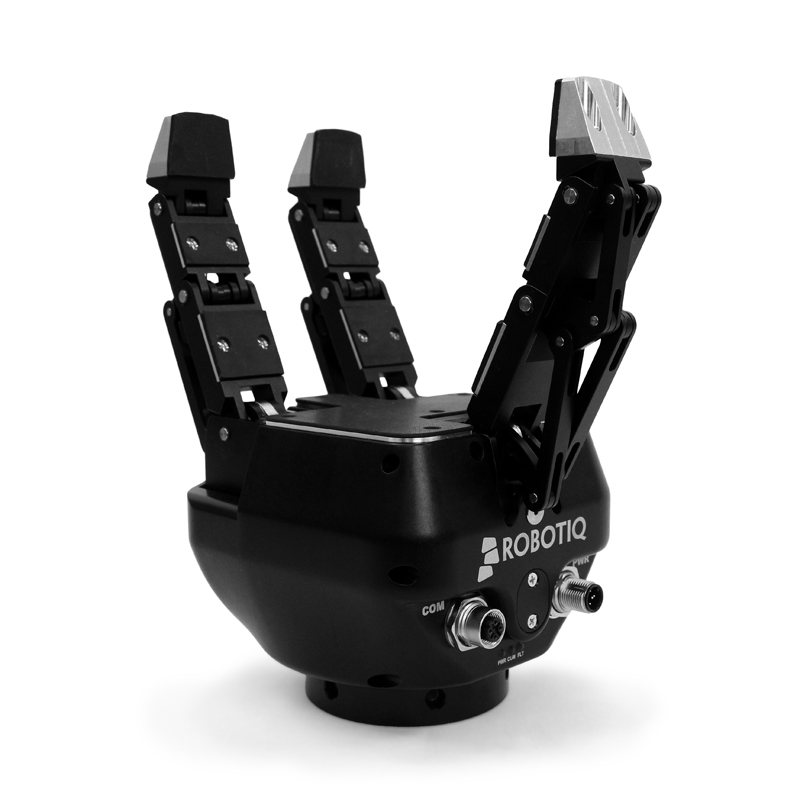
\includegraphics[width=0.7\textwidth]{Images/3-finger-robot-gripper-robotiq.jpg}
        \caption{3-Finger Adaptive Robot Gripper}
        \label{lbel:Robotiq3Finger}
    \end{subfigure}
    \begin{subfigure}{.3\linewidth}
        \centering
        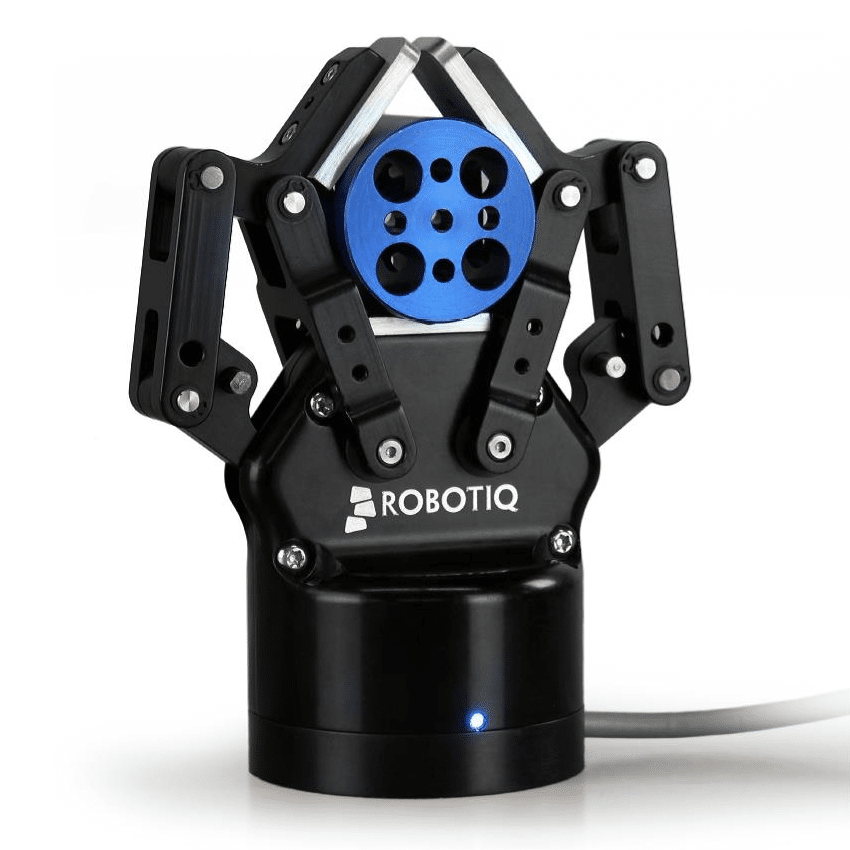
\includegraphics[width=0.7\textwidth]{Images/Robotiq-2-Finger-85-encompassing-grip.png}
        \caption{2F-85}
        \label{label:Robotiq85}
    \end{subfigure}
    \begin{subfigure}{.3\linewidth}
        \centering
        \includegraphics[width=0.7\textwidth]{Images/Hand£.png}           \caption{Hand-E}
        \label{label:Hand-E}
    \end{subfigure}
    \begin{subfigure}{.3\linewidth}
        \centering
        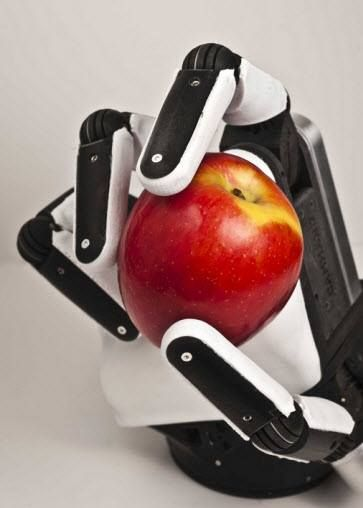
\includegraphics[width=0.7\textwidth]{Images/Sandia.jpg}        \caption{Sandia}
        \label{fig:Sandia}
    \end{subfigure}
    \begin{subfigure}{.3\linewidth}
        \centering
        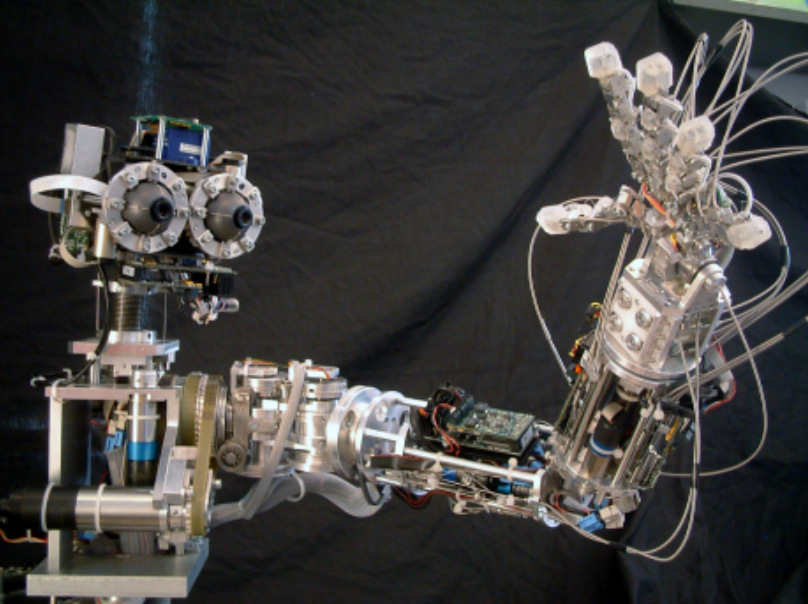
\includegraphics[width=0.7\textwidth]{Images/James.png}    \caption{James}
        \label{fig:James}
    \end{subfigure}
    \begin{subfigure}{.3\linewidth}
        \centering
        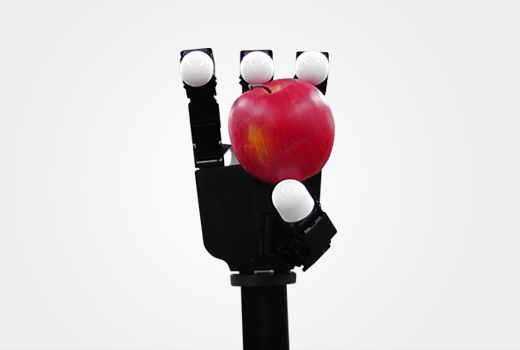
\includegraphics[width=0.7\textwidth]{Images/Allegro_Hand_flash_03.png}
        \caption{Allegro}
        \label{fig:Allegro}
    \end{subfigure}
    \begin{subfigure}{.3\linewidth}
        \centering
        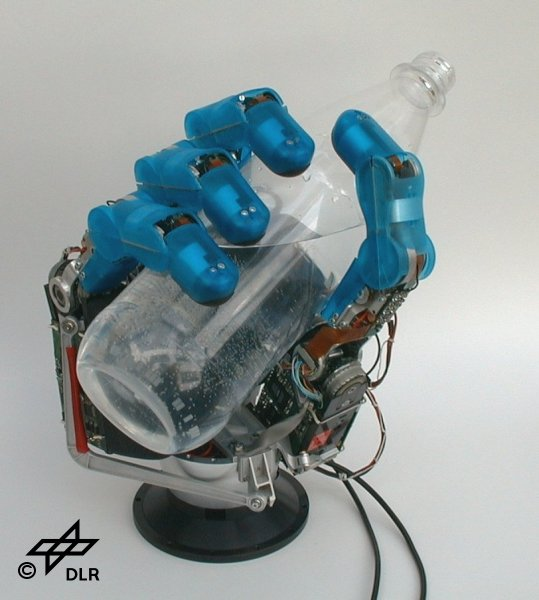
\includegraphics[width=0.7\textwidth]{Images/Hand-II-01.jpg}    \caption{DLR Hand II}
        \label{fig:DLR Hand II}
    \end{subfigure}
    \begin{subfigure}{.3\linewidth}
        \centering
        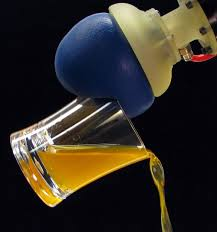
\includegraphics[width=0.7\textwidth]{Images/CoffeeBeanGripper.jpeg}    \caption{Coffee Bean Gripper}
        \label{fig:Coffee Bean Gripper}
    \end{subfigure}
\end{figure}

\subsection{Manipulators}
KUKA

\section{Grasp Sensing}

\subsection{Image}
Visual Camera
    RobotIQ, wrist camera
    
    
    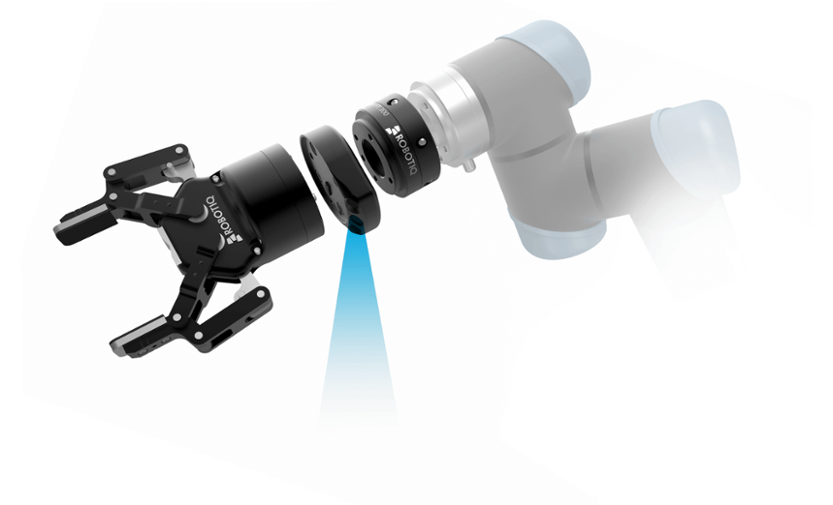
\includegraphics[width=0.2\textwidth]{Images/robotiq-vision-guided-robotic-hand-system.png}
Depth Camera
    APC 2016 Winners Delft

IR Sensing

\subsection{Tactile}
Hall Effect
Capacitive

\subsection{Joint Feedback}
Magnetic Encoders
Optical Encoders
Mechanical Encoders

\section{Actuation}
Actuation is a fundamental part of any manipulation system, the actuator is the component which enable the system to move. Broadly speaking the actuator will take some energy input, usually in the form of electrical or potential energy and convert that into kinetic energy. The actuator is essential for both moving the end effector into position and for the end effector to grasp the object. This section will look at the most common actuators used in robotic grippers to date, the advantages and disadvantages the trade off and the applications. This section will also look at actuation strategies, different ways to translate force or movement and examine the advantages and disadvantages of underactuated systems compared to fully actuated systems.

The first method of actuation examined is the DC motor. It is a very simple system where an electric potential input will cause a shaft to rotate. They are effective in a large range of sizes, inexpensive and efficient making them the most commonly used method of actuating any part of a robot. Despite this there are several disadvantages, DC motor produce maximum power and are most efficient at high speeds, this results in the use of gearboxs and other motion transmission methods which step down the speed while stepping up the torque. Although this trade off, more torque for less speed, is very advantageous for robotic applications there are inefficiencies and errors associated with these devices. Friction, noise and backlash are all problems which are introduced while making the system more expensive. Backlash in particular is a problem for robotic manipulation %% << H. Kawasaki and T. Komatsu, “Development of an anthropomorphic robot hand driven by built-in servo-motors,” in Proc. 3rd Int. Conf. ICAM, vol. 1, 1998, pp. 215–220.>>
, in order to maximize the number of poses which the manipulator can position and orientate its end effector in a manipulator generally has a large number of Degrees of Freedom (DOF). Similarly to maximise the flexibility of a gripper it also has a large number of DOF. In both cases these DOF are arranged in a relatively long open kinematic chain. The effect that blacklash and any other error between the desired and actual joint angle is that these error propigate and are amplified through the chain such that small relative errors caused by backlash at each joint causes a large absolute error in the position of the end effector.

A further disadvantage of using simple DC motors is the absence of a feedback mechanism. Generally the speed of a DC motor is determined by the voltage applied (neglecting the back emf in its coil) and the output torque is proportional to the current. Due to variations in these parameters it is difficult to determine the position of the motor at any particular time. Furturemore using the inputs to a DC motor as a way of determining the position of a robot joint is subject to error propigation since the volage input determines speed and in robotic manipulation we are generally interested in joint position. For example a small error in the estimation of the motor speed would cause the accumulation of a large error in the motor and therefore joint position over time.

Stepper Motors are another common method of actuation in robotics. They are similar in some ways to a simple DC motor but overcome some of the challenges while introducing a few also. Like a simple DC motor a stepper motor takes DC electricity as an input and produces kinetic energy in the form of a rotating shaft. The internal differences between a simple DC motor and a stepper motor is outside the scope of this document but in effect the mechanism by which a stepper motor operates allows it to be positionally controlled unlike its speed controlled brother the simple DC motor. This ability to control the position of the motor comes at the cost of requiring some kind of logic to control the motor, generally a micro-controller.

Beyond being able to set the position of a stepper motor there are several other advantages. Steppers motors exhibit holding torque which other DC motors cannot achieve, this means that aswell as being able to move a shaft it can also hold a shaft in position, a feature which is often used in manipulation applications.

Piezo electrics
Pneumatics
Artificial Muscles
Hydraulics

\subsection{Under Actuation}
Underactuation is a technique often used in robotics, among the mostly commonly sited reasons to choosing to underactuate a system is to reduce the number of actuators required \cite{UnderactuationReductionInActuactors}, to simplify the control and therefore computational overhead and to fully take advantage of the system's natural dynamic characteristics. 

A system is said to be underactuated if the number of dimensions in which it is free to move, i.e. its Degrees of Freedom (DOF) is more than the number of independently actuated joints. Most robots can be described by 

\begin{equation}
\ddot{q} = f_1(q,\dot{q},t) + f_2(q, \dot{q},t)u   
\end{equation}

where \(u\) is the control vector, \(t\) is time and the robot's state can be described by a vector of positions (\(q\)) and velocities(\(\dot{q}\)). In this more mathmatical formulation if 

\begin{equation}
    rank[f_2(q,\dot{q},t)] < dim[q]
\end{equation}

then the system is said to be underactuated.

More specific to robotic grippers underactuation can often be a desirable quality and give the grasper a degree of self adaptability.  

using elastic or flexible of elastic material to mechanically couple joints in the figure can allow the gripper to better adapt to the shape of an object and increase the chances of a successful grasp simply by carefully designing and utilising the physical embodiment of the hand.

\section{Grasping Strategies}
Sense Plan Act - Delft APC winners 20160

\section{Computation}

\section{Grasping Moving Objects}
Grasping dynamic objects adds another significant challenge to the manipulation problem but there are some examples of research and success in this area. The research to date can be broken down into three different levels of difficulty mainly based on how much is known about the object and its trajectory.

\begin{enumerate}
    \item Regular Object, controlled trajectory
    \item Irregular object, controlled trajectory
    \iten Regular object, uncontrolled trajectory
    \item Irregular object, uncontrolled trajectory 
\end{enumerate}

\begin{figure}
    \centering
        \begin{subfigure}
            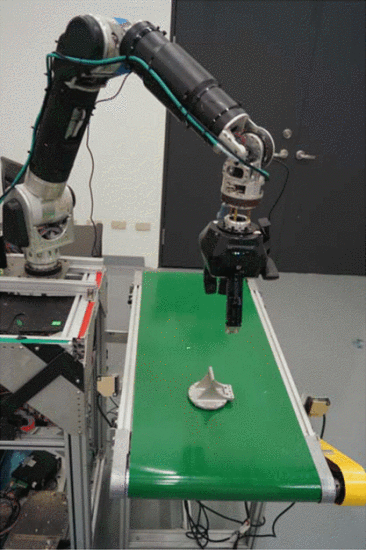
\includegraphics[]{Images/ConveyorBelt}
            \label{fig:Coffee Bean Gripper}
        \end{subfigure}
    \caption{Caption}
    \label{fig:my_label}
\end{figure}

\chapter{Exploration through simulation}

\section{Simulation Tools}

\subsection{Gazebo}
\subsection{MoveIt}
\subsection{RVIZ}
\subsection{ROS}

\section{Test Platforms}
Open Source, Community Developed, Custom Developed manipulators and grippers

\section{Methodology}
\subsection{Experimental Set-up}

Each platform tested on an established benchmark on a range of applications.
Creates a matrix of grippers against applications and performance.
Distil from this why each performed well or poorly and deduce what functionality, sensing, etc is need to perform well in each.

Next add extra sensing to the tested platforms, 2 categories of sensing, local and global (possibly 3, added tactile, added embedded camera, added global camera). Run tests on each gripper with added local sensing and added global sensing and evaluate the effect on performance.

\subsection{Evaluation Metrics}
Speed
Robustness
Accuracy
Range of Objects
Success Rate

\section{Results}


\section{Discussion}








\chapter{Computation}

Copy, Paste and modify the current draft of the botmark paper



Robotic competitions are fast becoming the \textit{de facto} standard for benchmarking robots in the field of service robotics. In this chapter, present a benchmarking suite is presented. It is designed specifically for evaluating the performance of computer platforms for performing functions common to these competitions, including manipulating tasks. An brief overview of computer benchmarking is firstly given along with popular robotic competitions relevant to service robotics. We take the RoboCup@Home competition as a prototypical exemplar of these  and develop a set of workloads based on the tests and functions that comprise it using a composite approach of the competing teams. The workloads are then run across a variety of computer platforms representative of the type commonly used and the results are presented. Other considerations are also investigated such as the power consumption, ease of development, I/O capabilities, price, size, etc. A wide variability is seen between computer systems. Finally, MORE HERE WHEN RESULTS ARE FOUND.


\section{Algorithms}

\section{Test Platforms}

Intel i5 Laptop 
Intel i7 
Parallela
Mini-ITX
Raspberry Pi
Intel Joule
NVIDIA P2597

\section{Methodology}
\subsection{Experimental Set-up}
\subsection{Evaluation Metrics}
Speed
Robustness
Accuracy
Range of Objects
Success Rate

\section{Results}


\section{Discussion}







\chapter{Tactile Sensing}
Talk about Tactile sensing, refer to literature review and the successful use of it on existing platforms.

\section{Experimental Rig}
Pictures of first and second gen rig

\section{Test sensors and material}

\section{Methodology}
\subsection{Experimental Set-up}
\subsection{Evaluation Metrics}


\section{Results}


\section{Discussion}







\chapter{Conclusion}


\section{Research Findings}


\subsection{Future Work}
Testing the effect of multiple embedded cameras on the grasping performance





\appendix
\chapter{Tables}

\begin{table}
\caption{Armadillos}
\label{arm:table}
\begin{center}
\begin{tabular}{||l|l||}\hline
Armadillos & are \\\hline
our	   & friends \\\hline
\end{tabular}
\end{center}
\end{table}

\clearpage
\newpage

\chapter{Figures}

\vspace*{-3in}

\begin{figure}
\vspace{2.4in}
\caption{Armadillo slaying lawyer.}
\label{arm:fig1}
\end{figure}
\clearpage
\newpage

\begin{figure}
\vspace{2.4in}
\caption{Armadillo eradicating national debt.}
\label{arm:fig2}
\end{figure}
\clearpage
\newpage

%% This defines the bibliography file (main.bib) and the bibliography style.
%% If you want to create a bibliography file by hand, change the contents of
%% this file to a `thebibliography' environment.  For more information 
%% see section 4.3 of the LaTeX manual.
\begin{singlespace}
\bibliography{main}
\bibliographystyle{plain}
\end{singlespace}


\end{document}

